\begin{figure}[htbp]
    \centering
    \begin{minipage}{0.45\textwidth}
        \centering
        
        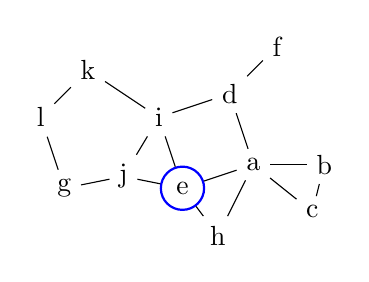
\begin{tikzpicture}[rotate = -90, scale = 0.6]
            % Nodes with manual coordinates
            \node (a) at (0.5,-1.5) {a};
            \node (b) at (0.5,0) {b};
            \node (c) at (1.5,-0.25) {c};
            \node (d) at (-1,-2) {d};
            \node[draw=blue, thick, circle] (e) at (1,-3) {e};
            \node (f) at (-2,-1) {f};
            \node (g) at (1,-5.5) {g};
            \node (h) at (2,-2.25) {h};
            \node (i) at (-0.5,-3.5) {i};
            \node (j) at (0.75, -4.25) {j};
            \node (k) at (-1.5,-5) {k};
            \node (l) at (-0.5,-6) {l};
            
            % Edges
            \draw (a) -- (b);
            \draw (a) -- (c);
            \draw (a) -- (d);
            \draw (a) -- (e);
            \draw (b) -- (c);
            \draw (e) -- (j);
            \draw (e) -- (h);
            \draw (d) -- (i);
            \draw (d) -- (f);
            \draw (j) -- (g);
            \draw (i) -- (j);
            \draw (i) -- (e);
            \draw (i) -- (k);
            \draw (g) -- (l);
            \draw (h) -- (a);
            \draw (l) -- (k);
        \end{tikzpicture}
    \end{minipage}
    \pause
    \begin{minipage}{0.45\textwidth}
        \centering
        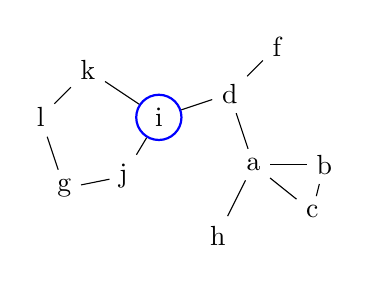
\begin{tikzpicture}[rotate = -90, scale = 0.6]
            % Nodes with manual coordinates
            \node (a) at (0.5,-1.5) {a};
            \node (b) at (0.5,0) {b};
            \node (c) at (1.5,-0.25) {c};
            \node (d) at (-1,-2) {d};
            \node (f) at (-2,-1) {f};
            \node (g) at (1,-5.5) {g};
            \node (h) at (2,-2.25) {h};
            \node[draw=blue, thick, circle] (i) at (-0.5,-3.5) {i};
            \node (j) at (0.75, -4.25) {j};
            \node (k) at (-1.5,-5) {k};
            \node (l) at (-0.5,-6) {l};
            
            % Edges
            \draw (a) -- (b);
            \draw (a) -- (c);
            \draw (a) -- (d);
            \draw (b) -- (c);
            \draw (d) -- (i);
            \draw (d) -- (f);
            \draw (j) -- (g);
            \draw (i) -- (j);
            \draw (i) -- (k);
            \draw (g) -- (l);
            \draw (h) -- (a);
            \draw (l) -- (k);
        \end{tikzpicture}
    \end{minipage}
    
    \pause
    \begin{minipage}{0.3\textwidth}
        \centering
        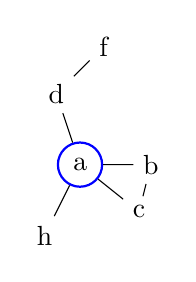
\begin{tikzpicture}[rotate = -90, scale = 0.6]
            % Nodes with manual coordinates
            \node[draw=blue, thick, circle] (a) at (0.5,-1.5) {a};
            \node (b) at (0.5,0) {b};
            \node (c) at (1.5,-0.25) {c};
            \node (d) at (-1,-2) {d};
            \node (f) at (-2,-1) {f};
            \node (h) at (2,-2.25) {h};

            
            % Edges
            \draw (a) -- (b);
            \draw (a) -- (c);
            \draw (a) -- (d);
            \draw (b) -- (c);
            \draw (d) -- (f);
            \draw (h) -- (a);
        \end{tikzpicture}
    \end{minipage}
    \pause
    \begin{minipage}{0.3\textwidth}
        \centering
        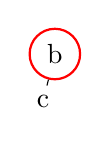
\begin{tikzpicture}[rotate = -90, scale = 0.6]
            % Nodes with manual coordinates
            \node[draw=red, thick, circle] (b) at (0.5,0) {b};
            \node (c) at (1.5,-0.25) {c};

            
            \draw (b) -- (c);
        \end{tikzpicture}
    \end{minipage}
\end{figure}